\section{Clustering}
\begin{itemize}
	\item Using the features engineered before to cluster instances
	\item Two different learning setups
	\begin{itemize}
		\item \textit{Per instance}: cluster data points/instances of quantified selfs. If multiple quantified selfs are available, we concatenate the datasets.
		\item \textit{Per person}: cluster different quantified selfs. Here, we consider all recorded instances of a person as a single data point, and we compare datasets/persons and cluster them. 
	\end{itemize}
\end{itemize}
\subsection{Distance Metrics}
\begin{itemize}
	\item We need different distance metrics per scenario
	\item We have to distinguish between feature-level and dataset-level
\end{itemize}
\subsubsection{Feature-level distance metrics}
\begin{itemize}
	\item For \textit{numerical} features, we can use the minkowski distance $\left(\sum_k \left|x_i^k - x_j^k\right|^q\right)^{1/q}$ which subsumes the Euclidean and Manhatten ($q=1$). However, we need to consider the scaling of the features (assumed to be equal)
	\item For \textit{categorical} features, we can use the Gower's similarity
	\begin{itemize}
		\item For binary attributes (called \textit{dichotomous}) $s(x_i^k, x_j^k)=1$ if $x_i^k$ and $x_j^k$ are present (i.e. are 1), else 0
		\item For categorical, we have $s(x_i^k, x_j^k)=\mathbbm{1}(x_i^k = x_j^k)$
		\item For numerical values in a range $R$, the Gower's similarity is $s(x_i^k, x_j^k)=1 - \frac{|x_i^k - x_j^k|}{R}$
		\item Similarity over multiple attributes is the mean of them
		\item Note that this is a similarity and not a distance (correlated by $\text{Similarity}\sim1/\text{Distance}$)
	\end{itemize}
\end{itemize}
\subsubsection{Dataset-level distance metrics}
\begin{itemize}
	\item We have to distinguish between datasets with and without temporal ordering
	\item \textbf{Non-temporal personal level distance metrics}: three different approaches possible
	\begin{enumerate}
		\item Summarize values per attribute over the entire dataset into a single number, as e.g. take the mean, min, max, stddev, etc. On these, we can use the same distance metrics as before
		\item Estimate parameters of a distribution that describes the dataset, such as a normal distribution with $\mathcal{N}(\mu, \sigma^2)$. On the parameters $\mu, \sigma^2$ we can apply the same distance metrics as before
		\item Compare the distributions of values for an attribute with a statistical test, such as the Kolmogorov Smirnov test. The distance metric would be $1-p$ where $p$ is the $p$-value returned by the test.
	\end{enumerate}
	\item \textbf{Temporal personal level distance metrics}: again, three different approaches
	\begin{enumerate}
		\item \textit{Feature-based}: extract features from the two time series, such as those from Section~\ref{sec:chapter_4_feature_engineering} (time and frequency domain).
		\item \textit{Model-based}: we try to fit a model on the two time series, and use those parameters to compare them. For example, we could use dynamical systems or similar
		\item \textit{Raw-data based} uses a distance per point.
		\begin{itemize}
			\item For example, it can assume a equal number of points in both datasets, and just takes e.g. the Euclidean Distance per time point
			\item Alternatively, we can also take a possible lag into account (shifted dataset). Then we compute the cross correlation coefficient $ccc(\tau, x_{qs_i}^{l}, x_{qs_j}^{l})=\sum_{k=-\infty}^{\infty} x_{k, qs_i}^{l} \cdot x_{k+\tau, qs_j}^{l}$. 
			\item Optimize $\tau$ by $\arg\min_{\tau} \sum_{k=1}^{p} \frac{1}{ccc\left(\tau, x_{qs_i}^{l}, x_{qs_j}^{l}\right)}$. Note that we have a single $\tau$ for all attributes
			\item \textbf{Dynamic Time Warping}: make best pairs of instances in the sequence to find minimum distance. Allows different frequencies of activities
			\begin{itemize}
				\item Two conditions for pairing: \\
				\textit{Monoticity condition}: time order has to be preserved. We cannot go ``back'' in time\\
				\textit{Boundary condition}: the first and last point must be aligned of the two time series
				\item Algorithm similar to finding shortest path in a graph.
				\begin{figure}[ht!]
					\centering
					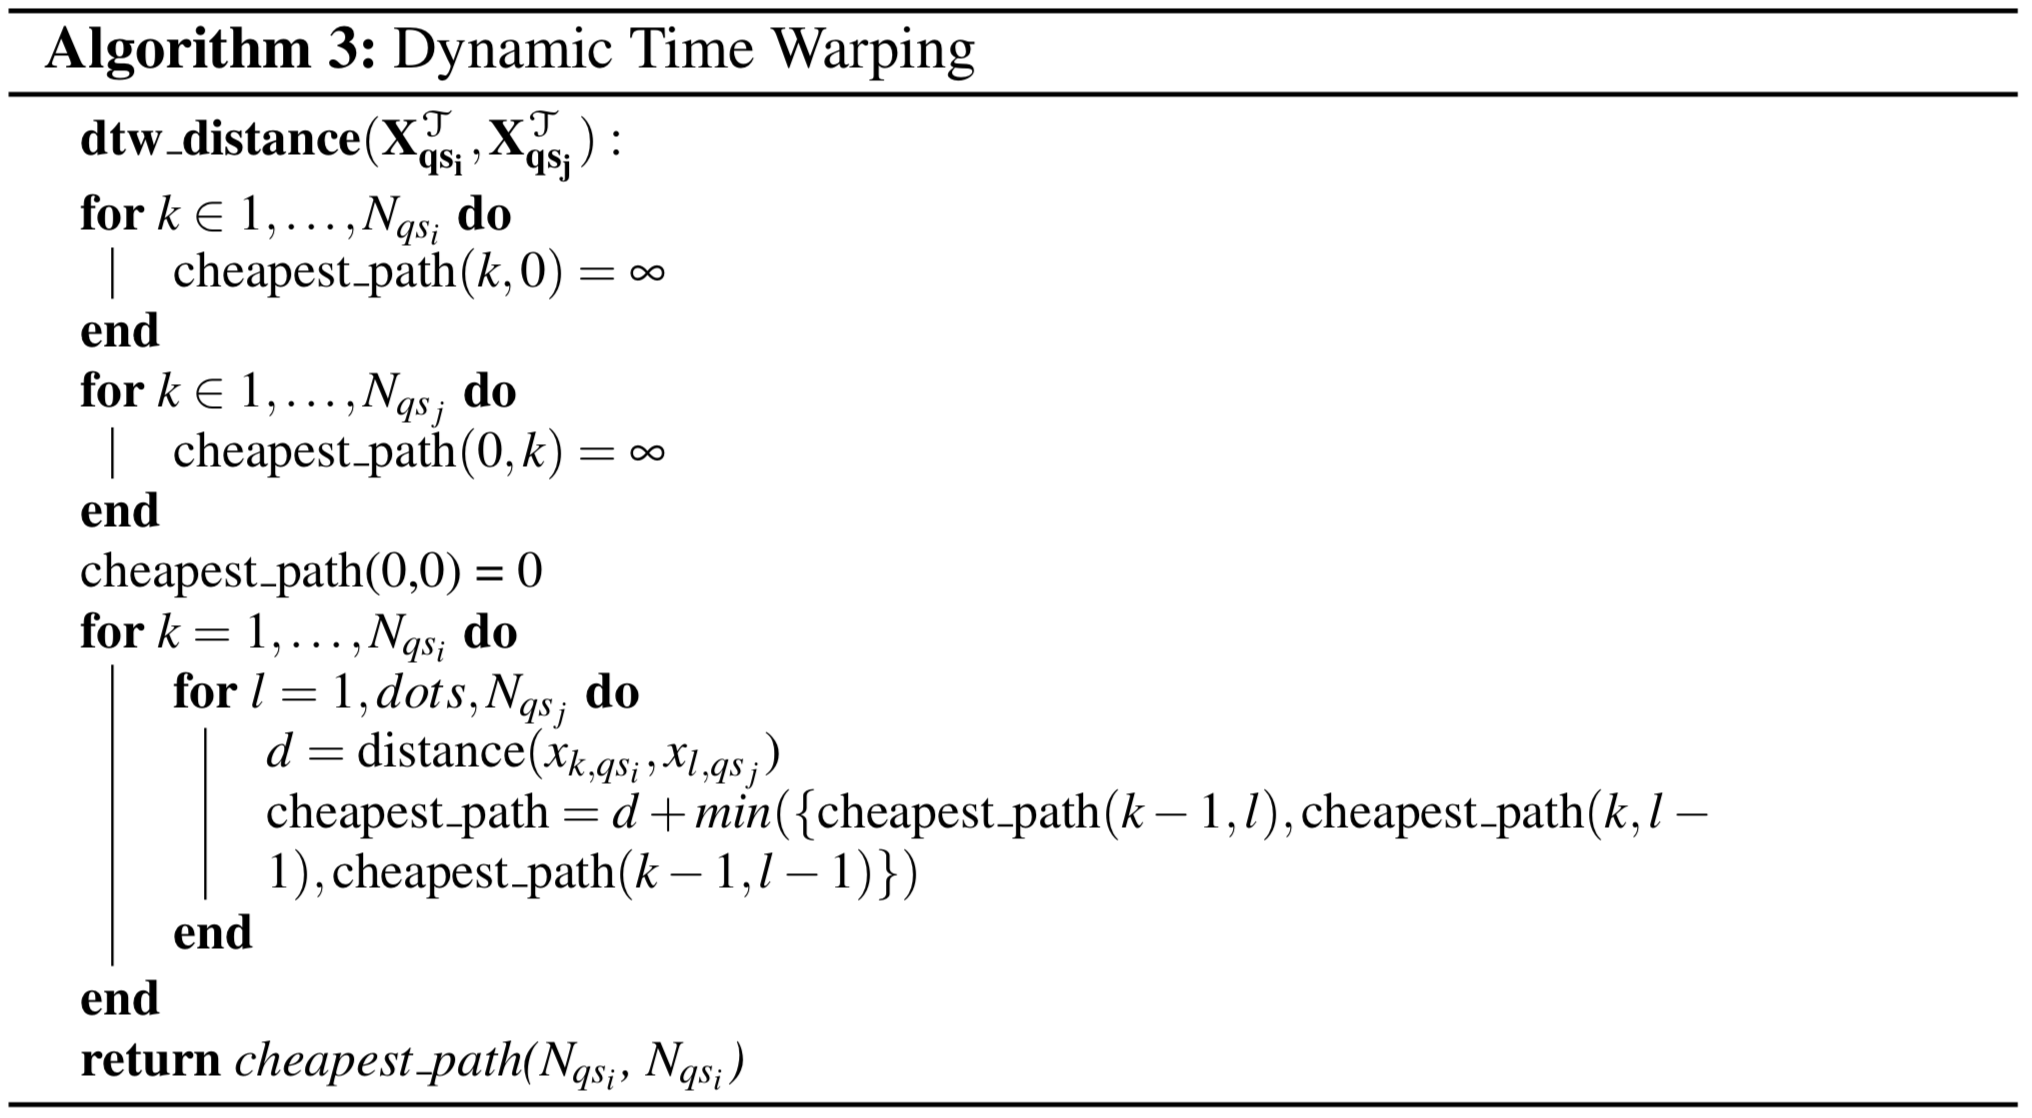
\includegraphics[width=0.5\textwidth]{figures/chapter_5_dynamic_time_warping.png}
					\caption{Algorithm of dynamic time warping}
				\end{figure}
				\item The drawbacks of this methods are that it is computational expensive ($\mathcal{O}(N\cdot M)$), and that the distance metric might not always be the best fit (i.e. should it be allowed to align the first point of sequence 1 with the last point of sequence 2?)
				\item \comment{For this algorithm, it helps more to practice it several times instead of writing it down in all details.}
			\end{itemize}
		\end{itemize} 
	\end{enumerate}
\end{itemize}
\subsection{Clustering approaches}
\begin{itemize}
	\item Overview of different clustering approaches
	\item \textbf{K-means}: define $k$ cluster means. A point is assigned to the cluster to which mean it is the closest. Means are updated by the assigned points.
	\begin{itemize}
		\item Using Silhoutte score to select best $k$/determine whether a clustering is good:
		\begin{equation*}
			\begin{split}
				\text{silhoutte} = \frac{\sum_{i=1}^{N}\frac{b(x_i) - a(x_i)}{\max(a(x_i), b(x_i)}}{N}\hspace{3mm} & \text{where}\hspace{2mm} a(x_i)=\frac{\sum_{\forall x_j \in C_l} d(x_i, x_j)}{|C_l|} \hspace{3mm} \text{(} x_i\in C_l\text{)}\\
				& \hspace{2mm}\text{and} \hspace{4mm} b(x_i) = \min_{C_m \neq C_l}\frac{\sum_{\forall x_j \in C_m} d(x_i, x_j)}{|C_m|}
			\end{split}
		\end{equation*}
		In text, the silhoutte score compares the average distance of a point with others within a cluster ($a(x_i)$) with the distance of points with the next closest cluster ($b(x_i)$). The larger the score, the better (between$[-1,1]$)
	\end{itemize}
	\item \textbf{K-medoids}: very similar to $k$-means, but we use actual points as cluster centers instead of artificial ones
	\begin{itemize}
		\item Choose new cluster means as the point with the minimum distance to all other points in the cluster
		\item More suitable if certain points in search space might not make sense
		\item For example, k-medoids is known to work better for person-level clustering
	\end{itemize}
\end{itemize}
\subsubsection{Hierarchical clustering}
\begin{itemize}
	\item Perform clustering in an iterative approach
	\item \textbf{Divisive clustering}: start with one cluster with all points in it, and in each step, perform one split
	\begin{itemize}
		\item Define the dissimilarity of a point to all other points in a cluster as the average distance $$\text{dissimilarity}(x_i, C)=\frac{\sum_{x_j\neq x_i \in C} \text{distance}(x_i, x_j)}{|C|}$$
		\item When creating a new cluster $C'$, we add the most dissimilar points (in order of dissimilarity) until a point is more dissimilar to the points in $C'$ than points in $C$. 
		\item If we have multiple clusters, we choose the cluster to split which has the greatest distance between any points in the cluster
	\end{itemize}
	\item \textbf{Agglomerative clustering}: start with all points in separate clusters, and merge them step by step. Merge decision can be based on different criteria (equal to distance metric between clusters):
	\begin{itemize}
		\item \textit{Single linkage}: merge the two clusters with the minimum distance between any two points
		$$d_{SL}(C_k, C_l) = \min\limits_{x_i \in C_k, x_j \in C_l} \text{distance}(x_i, x_j)$$
		\item \textit{Complete linkage}: merge the two clusters where the maximum distance between any two points is minimal
		$$d_{SL}(C_k, C_l) = \max\limits_{x_i \in C_k, x_j \in C_l} \text{distance}(x_i, x_j)$$
		\item \textit{Group average}: merge the two clusters with the average distance between all points is minimal
		$$d_{SL}(C_k, C_l) = \frac{\sum\limits_{x_i \in C_k, x_j \in C_l} \text{distance}(x_i, x_j)}{|C_k|\cdot |C_l|}$$
		\item \textit{Ward's criterion}: merge the two clusters where the increase of standard deviation by the combined cluster is minimal
		$$d_{SL}(C_k, C_l) = \sigma^2_{C_k \cup C_l} - \left(\sigma^2_{C_l} + \sigma^2_{C_k}\right)$$
	\end{itemize}
\end{itemize}
\subsubsection{Subspace clustering}
\begin{itemize}
	\item The problem of standard clustering algorithms for a huge number of features is that the distance between two points get uninformative (small distance in all features compared to big difference in only one feature). Hence, the clusters get less meaningful as well
	\item Better approach is therefore to look at subspaces in the feature space.
	\item Pseudo algorithm:
	\begin{enumerate}
		\item For all features, define intervals of the feature space. This leads to units $u={u_1, ..., u_p}$ where $u_i(l)$ is the lower-bound for attribute $i$ in this unit, and $u_h(l)$ the upper bound respectively. Note that units do not require to cover all features, but can look at subspaces only (same to setting lower bound to $-\infty$ and upper to $\infty$). 
		\item Determine selectivity of a unit as proportion of points in them. We call a unit ``dense'' if it contains more points/higher proportion than a certain threshold (hyperparameter).
		\item Units are connected to a cluster if they 
		\begin{itemize}
			\item share a common face which is defined as having the lower bound equals to an upper bound of another unit (or other way round), and the same upper and lower bound for all other attributes. 
			\item or when they share a unit to which they both have a common face.
		\end{itemize}
	\end{enumerate}
	\item In the end, we strive to find dense units using a combination of attributes to form clusters
	\item To reduce number of attributes, we can start to make units with a single attribute, and add more attributes iteratively based on some \textit{fancy} algorithm. After having found the units, we can create the clusters
\end{itemize}